\documentclass[tikz,border=10pt]{standalone}
% Shared look for every TikZ diagram. Load with \input{../../tools/tikz-style.tex}
\usepackage[T1]{fontenc}
\usepackage{lmodern}
\renewcommand{\sfdefault}{lmr}  % diagrams use the same serif as the text
\usetikzlibrary{arrows.meta, positioning, shapes.geometric, calc, fit, backgrounds}
\definecolor{cblue}{HTML}{4C78A8}
\definecolor{corange}{HTML}{F58518}
\definecolor{cgreen}{HTML}{54A24B}
\definecolor{cred}{HTML}{E45756}
\definecolor{cpurple}{HTML}{B279A2}
\definecolor{cgrey}{HTML}{6B6B6B}
\tikzset{
  every picture/.style={font=\sffamily, line width=1.2pt},
  box/.style={draw=#1, fill=#1!12, rounded corners=4pt, align=center, inner sep=7pt, minimum height=1.1cm},
  box/.default=cgrey,
  arrow/.style={-{Stealth[length=3mm]}, draw=cgrey, line width=1.4pt},
  title/.style={font=\sffamily\bfseries\Large},
  note/.style={font=\sffamily\small, text=cgrey, align=center},
}
\AtBeginDocument{\hyphenpenalty=10000 \exhyphenpenalty=10000}

\begin{document}
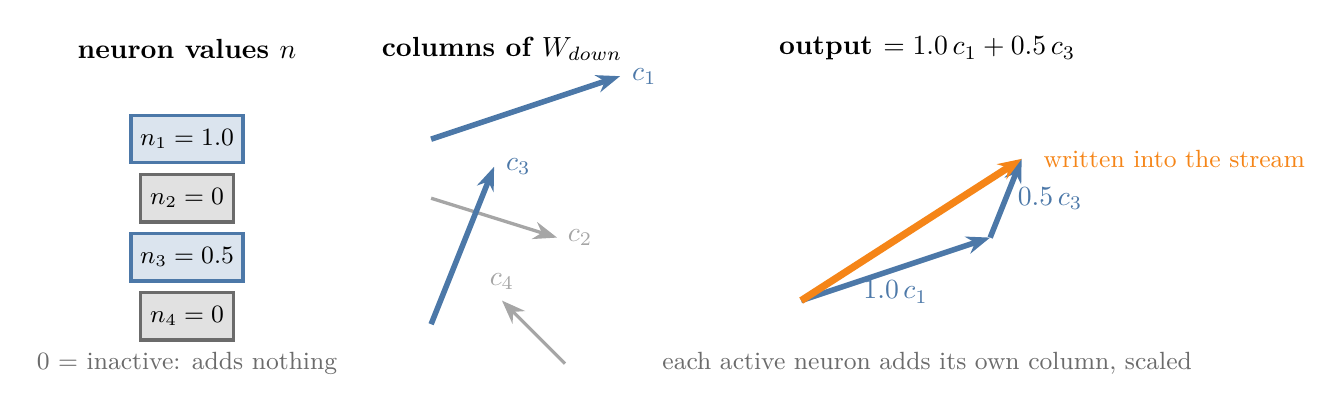
\begin{tikzpicture}[>={Stealth[length=3mm]}]
  % neuron values
  \node[font=\sffamily\bfseries] at (1.2,4.4) {neuron values $n$};
  \foreach \v/\c [count=\k] in {1.0/cblue, 0/cgrey, 0.5/cblue, 0/cgrey} {
    \node[draw=\c, fill=\c!20, minimum width=1.0cm, minimum height=0.6cm, font=\sffamily\small] (n\k) at (1.2,4.0-0.75*\k) {$n_\k = \v$};
  }
  \node[note] at (1.2,0.4) {0 = inactive: adds nothing};
  % columns
  \node[font=\sffamily\bfseries] at (5.2,4.4) {columns of $W_{\text{down}}$};
  \draw[->, cblue, line width=2pt] (4.3,3.25) -- ++(2.4,0.8) node[right, font=\sffamily] {$c_1$};
  \draw[->, cgrey!60, line width=1.2pt] (4.3,2.5) -- ++(1.6,-0.5) node[right, font=\sffamily] {$c_2$};
  \draw[->, cblue, line width=2pt] (4.3,0.9) -- ++(0.8,2.0) node[right, font=\sffamily] {$c_3$};
  \draw[->, cgrey!60, line width=1.2pt] (6.0,0.4) -- ++(-0.8,0.8) node[above, font=\sffamily] {$c_4$};
  % sum
  \node[font=\sffamily\bfseries] at (10.6,4.4) {output $= 1.0\,c_1 + 0.5\,c_3$};
  \coordinate (o) at (9.0,1.2);
  \draw[->, cblue, line width=2pt] (o) -- ++(2.4,0.8) coordinate (a) node[midway, below, font=\sffamily] {$1.0\,c_1$};
  \draw[->, cblue, line width=2pt] (a) -- ++(0.4,1.0) coordinate (b) node[midway, right, font=\sffamily] {$0.5\,c_3$};
  \draw[->, corange, line width=2.6pt] (o) -- (b);
  \node[note, anchor=west, text=corange] at ([xshift=4pt]b) {written into the stream};
  \node[note] at (10.6,0.4) {each active neuron adds its own column, scaled};
\end{tikzpicture}
\end{document}
